\section{Aufgabenstellung}
Es ist ein Programm zu entwerfen, welches Audiodateien einliest und dateiweise die beiden Stereo-Kanäle miteinander korreliert. Es sollen Maßzahlen entworfen und berechnet werden, die wesentliche charakteristische Eigenschaften der Korrelationsfunktion, insbesondere den Anteil dominanter Komponenten und deren Abklingverhalten, widerspiegeln. Dafür sind Audiosignale aufzunehmen, bezüglich der verwendeten Maße zu klassifizieren und entsprechend ihrer Klassifzierung systematisch abzuspeichern.
%%%%%%%%%%%%%%%%%%%%%%%%%%%%%%
\section{Motivation}
Im Jahr 2022 werden 500 Milliarden internetfähige Geräte erwartet, die mit einander kommunizieren sollen. Das führt zu extrem hohen Datenmengen, die in kürzestmöglicher Zeit von A nach B transportiert werden müssen. Große Herausforderungen bestehen darin, dass man sehr kurze Verzögerungszeiten und eine hohe Widerstandsfähigkeit garantieren muss. Idealerweise benötigen die Geräte wenig Energie. Ein Ansatz zur Lösung dieses Problems ist die Netzwerkcodierung.\newline
In bestimmten Szenarien ist eine große Anzahl an Geräten mit Sensorik zu Erfassung der Umgebung mit hohen Anforderungen an die Netzwerkkapazität zur Übertragung der erfassten Daten verbunden. Es stellt sich die Frage, wie viele Sensoren für eine ausreichend genaue Abbildung benötigt werden. Da die Quellen teilweise korrelierte Datenströme erzeugen, lässt sich die zu übertragende Gesamtdatenmenge reduzieren, was durch eine geeignete Kombination von Netzwerkcodierung mit Methoden des Compressed Sensing erreicht werden soll.

%%%%%%%%%%%%%%%%%%%%%%%%%%%%%%
\section{Theoretische Vorbetrachtung}
\subsection{Kreuzkorrelationsfunktion}
Die Basis f"ur die Bemessung der aufgenommenen Audiosignale bildet die sogenannte Kreuzkorrelationsfunktion (KKF). Wie in der Aufgabenstellung schon beschrieben werden an ihr die Bemessungsparameter festgelegt. Aufgrund der verschiedenen Blockl"angen und der Masse an Daten, die korreliert werden sollen muss die Berechnung der KKF effizient und zeitsparend implementiert werden. Im Folgenden Abschnitt wird die KKF kurz theoretisch eingef"uhrt und das das mathematische Konzept erkl"art, auf dem die effiziente Berechnung der KKF beruht.
\\\\
Zuerst haben wir f"ur die KKF eine Funktion genutzt, die zur Berechnung Summen verwendete. Dabei ergab sich, dass die Berechnung zu langsam war. In der nun vorliegenden Octave-Version wird die KKF im Frequenzbereich berechnet.
\subsubsection{Berechnungsvorschrift}
Die KKF ist als aus zwei verschiedenen Funktionen gebildeter Erwartungswert definiert. Hier werden die Formeln allgemein f"ur die Korrelation der Prozesse \textbf{X} und \textbf{Y} angegeben. 

\begin{align}
\psi_{\textbf XY}(t_1, t_2) = E\lbrace\textbf{X}(t_1)\cdot\textbf{Y}(t_2)\rbrace
\end{align}
Reale aufgenommene Audiosignale s(t), die hier mit durch die KKF verrechnet werden, sind in jedem Fall Energiesignale, da sie rein reell sind, einen begrenzten Wertebereich haben und nach einer bestimmten Zeit enden.

\begin{align}
Signalenergie := \int_{-\infty}^{\infty} s^2(t) \,dt < \infty
\end{align}

\noindent Da die aufgenommenen Audiosignale zeit-diskrete Energiesignale sind wird hier auch nur die zeit-diskrete Kreuzkorrelation beschrieben. F"ur zeit-diskrete Energiesignale ergibt sich die folgende Berechnungsvorschrift, wobei x(n) und y(n) Realisierungen der Prozesse \textbf{X} und \textbf{Y} sind.

\begin{align}
\boxed{\psi_{\textbf {XY}}^E(k) = \sum_{n = -\infty}^{\infty} x(n) \cdot y(n+k)}
\end{align}
vgl. [ISV] S. 84 folgende

\subsubsection{Kreuzkorrelation im Frequenzbereich und Faltungssatz}
Am Anfang unserer Arbeit haben wir uns mit der Berechnung der Kreuzkorrelation besch"aftigt. Da die Bildung der Summe der Multiplikation von x(n) und y(n+k) sehr rechenaufw"andig ist, haben wir nach schnelleren M"oglichkeiten gesucht die KKF der beiden Signale zu berechnen. Eine geeignet M"oglichkeit ist die Berechnung der KKF im Frequenzbereich. F"ur die Berechnung der KKF im Frequenzbereich macht man sich die "Ahnlichkeit der KKF zur Faltung und den Faltungssatz zunutze.

\paragraph{KKF als Faltung}
%hier herrscht noch unsicherheit vor, ich habe nur die Formel für den kont. Fall
\textbf{\\\\Zeit-kontinuierlicher Fall:}
\begin{align}
\psi_{\textbf {XY}}^E(\tau) = x(-\tau) * y(\tau)
\end{align}
\textbf{Zeit-diskreter Fall:}
\begin{align}
\psi_{\textbf {XY}}^E(k) = x(-k) * y(k)
\end{align}
[ISV] Formel (2.217) S.89

\paragraph{Faltungssatz in Verbindung mit KKF}

Wir schreiben zuerst die die KKF als Faltung. Danach transformieren wir die Faltung in den Frequenzbereich. Durch geschicktes Erweitern und Substitution findet man einen Ausdruck, um die KKF im Frequenzbereich zu berechnen.

\begin{align}
\psi(t) \  \; &= x(-t) * y(t) = \int_{-\infty}^{\infty} x(-\tau) \cdot y(t-\tau)\,d\tau\\\\
\underline \Psi(\omega) &=\int_{-\infty}^{\infty} x(-t) * y(t) \cdot e^{-j\omega t} \,dt\\&=\int_{-\infty}^{\infty} \left[ \int_{-\infty}^{\infty} x(-\tau) \cdot y(t-\tau)\,d\tau \right] \cdot e^{-j\omega (t - \tau + \tau)} \,dt\\&=\int_{-\infty}^{\infty} x(-\tau) \cdot e^{j\omega(-\tau)} \underbrace{ \left[ \int_{-\infty}^{\infty} y(t-\tau) e^{-j\omega (t - \tau)} \,dt \right]}_* \,d\tau
\end{align}
Durch Substitution von $(t-\tau)$ durch $t'$ ergibt sich * zur Fourier-transformierten $ \underline{Y}(\omega)$ von y(t). Der restliche Ausdruck wird durch das positive Vorzeichen in der e-Funktion zur komplex konjugierten Transformierten $ \underline{X}^*(\omega)$ der Funktion x(t).
\\\\
Die KKF l"asst sich im Frequenzbereich also als

\begin{align}
\boxed{\underline \Psi(\omega) = \underline{X}^*(\omega) \cdot \underline{Y}(\omega)}
\end{align}
schreiben.
\\vgl. [ISV] S.180
\\\\
Wenn man nun die KKF im Frequenzbereich zeitsparend durchf"uhren will, muss man die FFT f"ur x(k) und y(k) (dabei $k \in \mathbb{N}^+_0$) der L"ange N durchf"uhren. Dabei muss man beachten, dass bei der FFT ein Linienspektrum ergibt. Die FFT beruht vor allem auch auf der Annahme, dass sich die N diskreten Werte periodisch wiederholen. Durch die IFFT von $ \underline \Psi(\omega)$ ergibt sich also die periodische KKF $\tilde{\psi}(t)$.\\vgl. [ISV] S.135\\\\Die periodische KKF $\tilde{\psi}(t)$ ist in unserem Projekt zudem die bessere Wahl. Berechnet man die KKF im Frequenzbereich wird durch die implementierten Funktionen von Octave, so wie von Python, sogenanntes "Zero-Padding" durchgeführt. Vorstellen kann man sich das als auffüllen der Daten mit N Werten $=0$ an jeweils den Rändern einer der beiden Funktionen, da durch die Verschiebung über den Rand der anderen hinausragt.

\begin{figure}[h] 
  \centering
     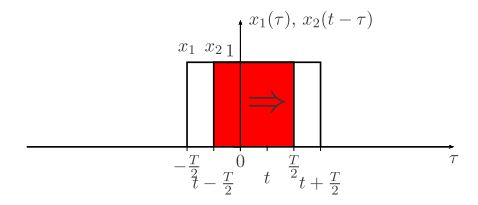
\includegraphics[width=0.7\textwidth]{Faltung.jpg}
  \caption{Anschauliches Beispiel zur Faltung}
  \label{fig:Bild1}
\end{figure}
vgl. [NT] Seite 28\\
Wie man auf dem Bild erkennen kann ist die Funktion $x_2$ soweit verschoben, dass sie über den rechten Rand der Funktion $x_1$ hinausragt. Wenn man die beiden Rechtecksignale als Bereiche sieht in denen echte Funktionswerte liegen, würde nun auf der positiven x-Achse ab $T/2$ mit Nullen aufgefüllt werden. Dadurch bekommt die KKF automatisch ein Abklingverhalten an ihren Rändern, das nur durch die begrenzte Anzahl an Werten verursacht wird. Die Korrelation nimmt an den Rändern nicht zwingend ab. Durch dieses Abklingverhalten würden unsere Ergebnisse also abgefälscht werden. Die periodische KKF ist also aussagekräftiger, da unser reales Signal in jedem Fall an den Rändern der korrelierten Blöcke nicht auf Null abklingt.Wenn man die periodische KKF im Zeitbereich berechnen möchte, müsste man an den Rändern der Funktionen nochmal die Funktion $x_1$ anhängen.
\subsection{Maßzahlen}
\small\textit{verfasst von Florian Roth}
\normalsize
\\ Im Anschluss an diese Arbeit gilt es zu untersuchen, in wie fern die aufgenommenen Signale geeignet sind um mittels Netzwerkcodierung und Compressed Sensing unter Einsparung von Datenverkehr versendet werden können. 
\\ Um das für eine große Anzahl an Signalen überhaupt möglich zu machen, ist es erforderlich die untersuchten Signale anhand von  bestimmten Eigenschaften zu klassifizieren. Damit ein einfacher Vergleich mehrerer Signale schnell möglich ist, bietet es sich an diese Eigenschaften als Zahlenwert auszudrücken. 
\\ Die beschriebenen Eigenschaften sind entweder physikalischer Natur oder versuchen die Form der Kreuzkorrelation zu charakterisieren. Dabei wurde darauf geachtet, wenn möglich normierte Größen zu verwenden um die Vergleichbarkeit zwischen Signalen unterschiedlicher Abtastrate und Zeitdauer aufrecht zu erhalten. 
\\ Beim Entwerfen solcher Maßzahlen besteht die Schwierigkeit darin, möglichst viel aussagekräftige Information dahingehend zu vereinfachen, dass eine Überführung in eine Zahl überhaupt möglich ist. Gleichzeitig darf durch die Vereinfachung nicht die Aussagefähigkeit der Maßzahl zerstört werden, also die Möglichkeit auf eine Eigenschaft des Signals anhand des Zahlenwertes zurück zu schließen. Aufgrund dieser Anforderungen sind im Verlauf dieser Arbeit mehrere Maßzahlen entstanden, von denen einige im weiteren Prozess wieder verworfen wurden. 
\\Die Bedeutung und Berechnung der finalen Maßzahlen wird hier kurz vorgestellt. 
\subsubsection{ripple}
Die Maßzahl \textit{ripple} trifft eine Aussage über die Energieverteilung im Signal. Zur Berechnung wird die Energie, die die obersten fünf Perzentile der berechneten Werte enthalten, ins Verhältnis zur Gesamtenergie gesetzt. 
\begin{align*}
ripple = \frac{\sum_{\text{der obersten 5 Perzentile}}x_{i}^2}{\sum_{i=1}^{N}x_{i}^2}
\end{align*}
\textit{ripple} kann Werte zwischen 0 und 1 annehmen, wobei $ripple = 0$ bedeutet, dass es sich um eine konstante Funktion handelt, während $ripple = 1$ auf einen einzelnen Impuls schließen lässt.
\subsubsection{sigma}
Ziel war es eine Maßzahl zu finden, die eine Aussage über die Verteilung der größten Werte der Kreuzkorrelation liefert. In einer ersten Version des Programmes wurde die in Octave intigrierte Funktion \textit{xcorr} verwendet, die zero-padding nutzt, wenn sie die Signale im Zeitbereich zueinander verschiebt. Dadurch fiel die KKF zu den Seiten schnell ab und die Hüllkurve erinnerte stark an eine Glockenkurve. Ein Maß für die ,,Breite'' einer Glockenkurve stellt das \textit{sigma} im Exponenten der $e$-Funktion dar. 
\\Auch nach dem Umstellen auf eine andere KKF-Berechnung, bei der durch periodisches Aneinandersetzen der Signale kein Abfall auf Null zu den Rändern stattfindet, konnte in einem Großteil der Korrelationshüllkurven weiterhin eine Glockenkurvenform vorgefunden werden, allerdings nun mit Gleichanteil. Um die gewünschte Maßzahl \textit{sigma} aus den numerisch vorliegenden Werten zu erhalten, muss ein mathematischer Ausdruck für die Hüllkurve gefunden werden. Die Hülllkurve \textit{envelope} wiederum erhält man durch Amplituden-Demodulation der KKF. Dabei wird das Signal gleichgerichtet und auf ein Tiefpassfilter gegeben. Der Filter wird in dieser Arbeit im Frequenzbereich realisiert mit einer von der zeitlichen Länge des Signals $t_{Signal}$ abhängigen Grenzfrequenz $f_{c} = \frac{20}{t_{Signal}}$. Bei dem Zahlenwert $20$ handelt es sich um einen experimentell bestimmten Wert. 
\begin{align*}
envelope = IDFT\lbrace DFT\lbrace|\psi_{\text{XY}}(n)|\rbrace\cdot\text{H}_{\text{TP}}\rbrace
\end{align*}
Für die Hüllkurve \textit{envelope} wird nun mittels Methode der kleinsten Quadrate eine Regressionsrechnung auf die vermutete Glockenkurvenfunktion vorgenommen. Die Funktionsvorschrift lautet dabei
\begin{align*}
y = a\cdot e^{-\frac{(x-\mu)^2}{2\sigma^2}}+b
\end{align*}
Mit den zu bestimmenden Konstanten $a$, $b$, $\mu$ und $\sigma$. Mit dem erhaltenen Wert für $\sigma$ lässt sich keine Aussage über den Anteil der Fläche der Hüllkurve in den Grenzen $\mu-\sigma$ bis $\mu+\sigma$ treffen. Das liegt an dem Gleichanteil und keiner Verknüpfung mit der Amplitude $a$ wie bei der Gauss'schen Glockenkurve. Sehr wohl stellt $\sigma$ allerdings ein Maß für die Breite des peaks rund um den Nullpunkt der Korrelation dar. Die Angabe erfolgt in Sekunden. 
\subsubsection{timeDiff}
Der Parameter \textit{timeDiff} gibt den zeitlichen Versatz der Stereokanäle zueinander wieder. Dazu wird der Indexwert $i$ des Maximums der Kreuzkorrelation bestimmt und anhand der Samplingrate $r$ die Zeitdifferenz zum Nullpunkt ($\lambda = 0$) berechnet.
\begin{align*}
\Delta t = \frac{\Delta i}{r}
\end{align*}
\subsubsection{exp und area}
Da die Regression auf eine Glockenkurve nicht für alle Signale sinnvoll ist, war eine Maßzahl gefordert, die zumindest den Abfall der Gesamtheit aller Amplituden angibt. Dazu wurden die diskreten Werte der Korrelation betragsmäßig absteigend geordnet. Anschließend wurde wieder eine Regressionsrechnung mit Hilfe der Methode der kleinsten Quadrate angewandt. Dabei handelt es sich nun um eine einfache abfallende e-Funktion
\begin{align*}
y = e^{-c \cdot x}
\end{align*}
wobei der ausgegebene Parameter \textit{exp} der ermittelten Konstante $c$ entspricht, normiert auf die Länge des Signals. Bei Vergleich der Regressionskurve mit der ursprünglichen Funktion fällt auf, dass diese nur schlecht angenähert wird. Auf ein modifizieren der Funktion, beispielsweise durch Addition eines Gleichanteils, wird jedoch verzichtet, da die Verrechnung der zusätzlichen Parameter zu einer aussagekräftigen Maßzahl nicht glückte. Ein Maß für den geforderten Abfall stellt auch die einfache e-Funktion dar. 
\\Um einen alternativen Parameter zu bestimmen wird die Fläche unter der Kurve berechnet und auf die Länge des Signals normiert. 
\begin{align*}
area = \frac{1}{N_{\text{samples}}} \sum_{n=1}^{N_{\text{samples}}} |\psi_{\text{XY}}(n)|
\end{align*}
Eine Normierung auf den Maximalwert erfolgt schon beim Berechnen der Kreuzkorrelation. Dadurch kann \textit{area} nur Werte zwischen $0$ und $1$ annehmen. Je kleiner \textit{area}, desto steiler fallen die Amplituden ab. 
\\Trotz der erfolgreich ermittelten Maßzahl \textit{area}, berechnet das Programm weiterhin den Parameter \textit{exp}, denn dieser lässt sich leicht modifizieren und kann somit noch an Aussagekraft hinzu gewinnen. 

\subsection{Gauß-Regression}

%%%%%%%%%%%%%%%%%%%%%%%%%%%%%%
\section{Verfügbare Technik}
\subsection{Software}
Softwareseitig haben wir Octave benutzt. Als freie Alternative zu Matlab vereint Octave gute Performance, syntaktische Gleichheit zu Matlab, sowie kostenfreie Benutzung unter einem Dach. Im Vergleich mit Python haben wir festgestellt, dass die Geschwindigkeit aufwendiger Rechnungen, wie der Korrelation, bei Python schlechter ist. Somit haben wir uns für Ocatve entschieden. Um unseres selbstgeschriebenes Programm zu verifizieren haben wir eine Autokorrelation durchgeführt und diese mit der von Audactity berechneten AKF verglichen. Wir sind dabei zu dem Ergebnis gekommen, dass unser Programm funktioniert. Zur Aufnahme der Audiosignale haben wir ebenfalls die Software Audacity benutzt.
\subsection{Hardware}
Uns standen zwei hochwertige Kondensatormikrofone (M5 Matched Pair Compac 1/2" Cardioid Condenser Microphones von Rode) zur Verfügung. Diese Mikrofone sind für dieses Projekt besonders geeignet, da durch die Abstimmung (matched pair) nur die Unterschiede im Signal vor der Aufnahme Einfluss auf die Korrelation haben. Da es sich um Mikrofone mit Nierencharakteristik handelt, ist jedoch zu beachten, dass es sich bei den Aufnahmen um Gerichtete handelt und nicht wie bei Mikrofonen mit Kugelcharakteristik von einer Abbildung des gesamten gemessenen Raumes ausgegangen werden kann. Für die Digitalisierung der Signale stand uns ein hochwertiges Audio-USB-Interface (Scarlett 2i2 von Focusrite) zur Verfügung. Die Aufnahmen wurden in .wav gespeichert und sind somit verlustfrei. Außerdem konnten wir ein Stativ mit einer Mikrofonschiene verwenden, wodurch die Mikrofone konstanten Abstand hatten. Zur Erzeugung eines reproduzierbaren Klangsignales wurde eine portable Bluetooth-Anlage (Soundlink III von Bose) verwendet.

\begin{figure}[ht!]
  \centering
  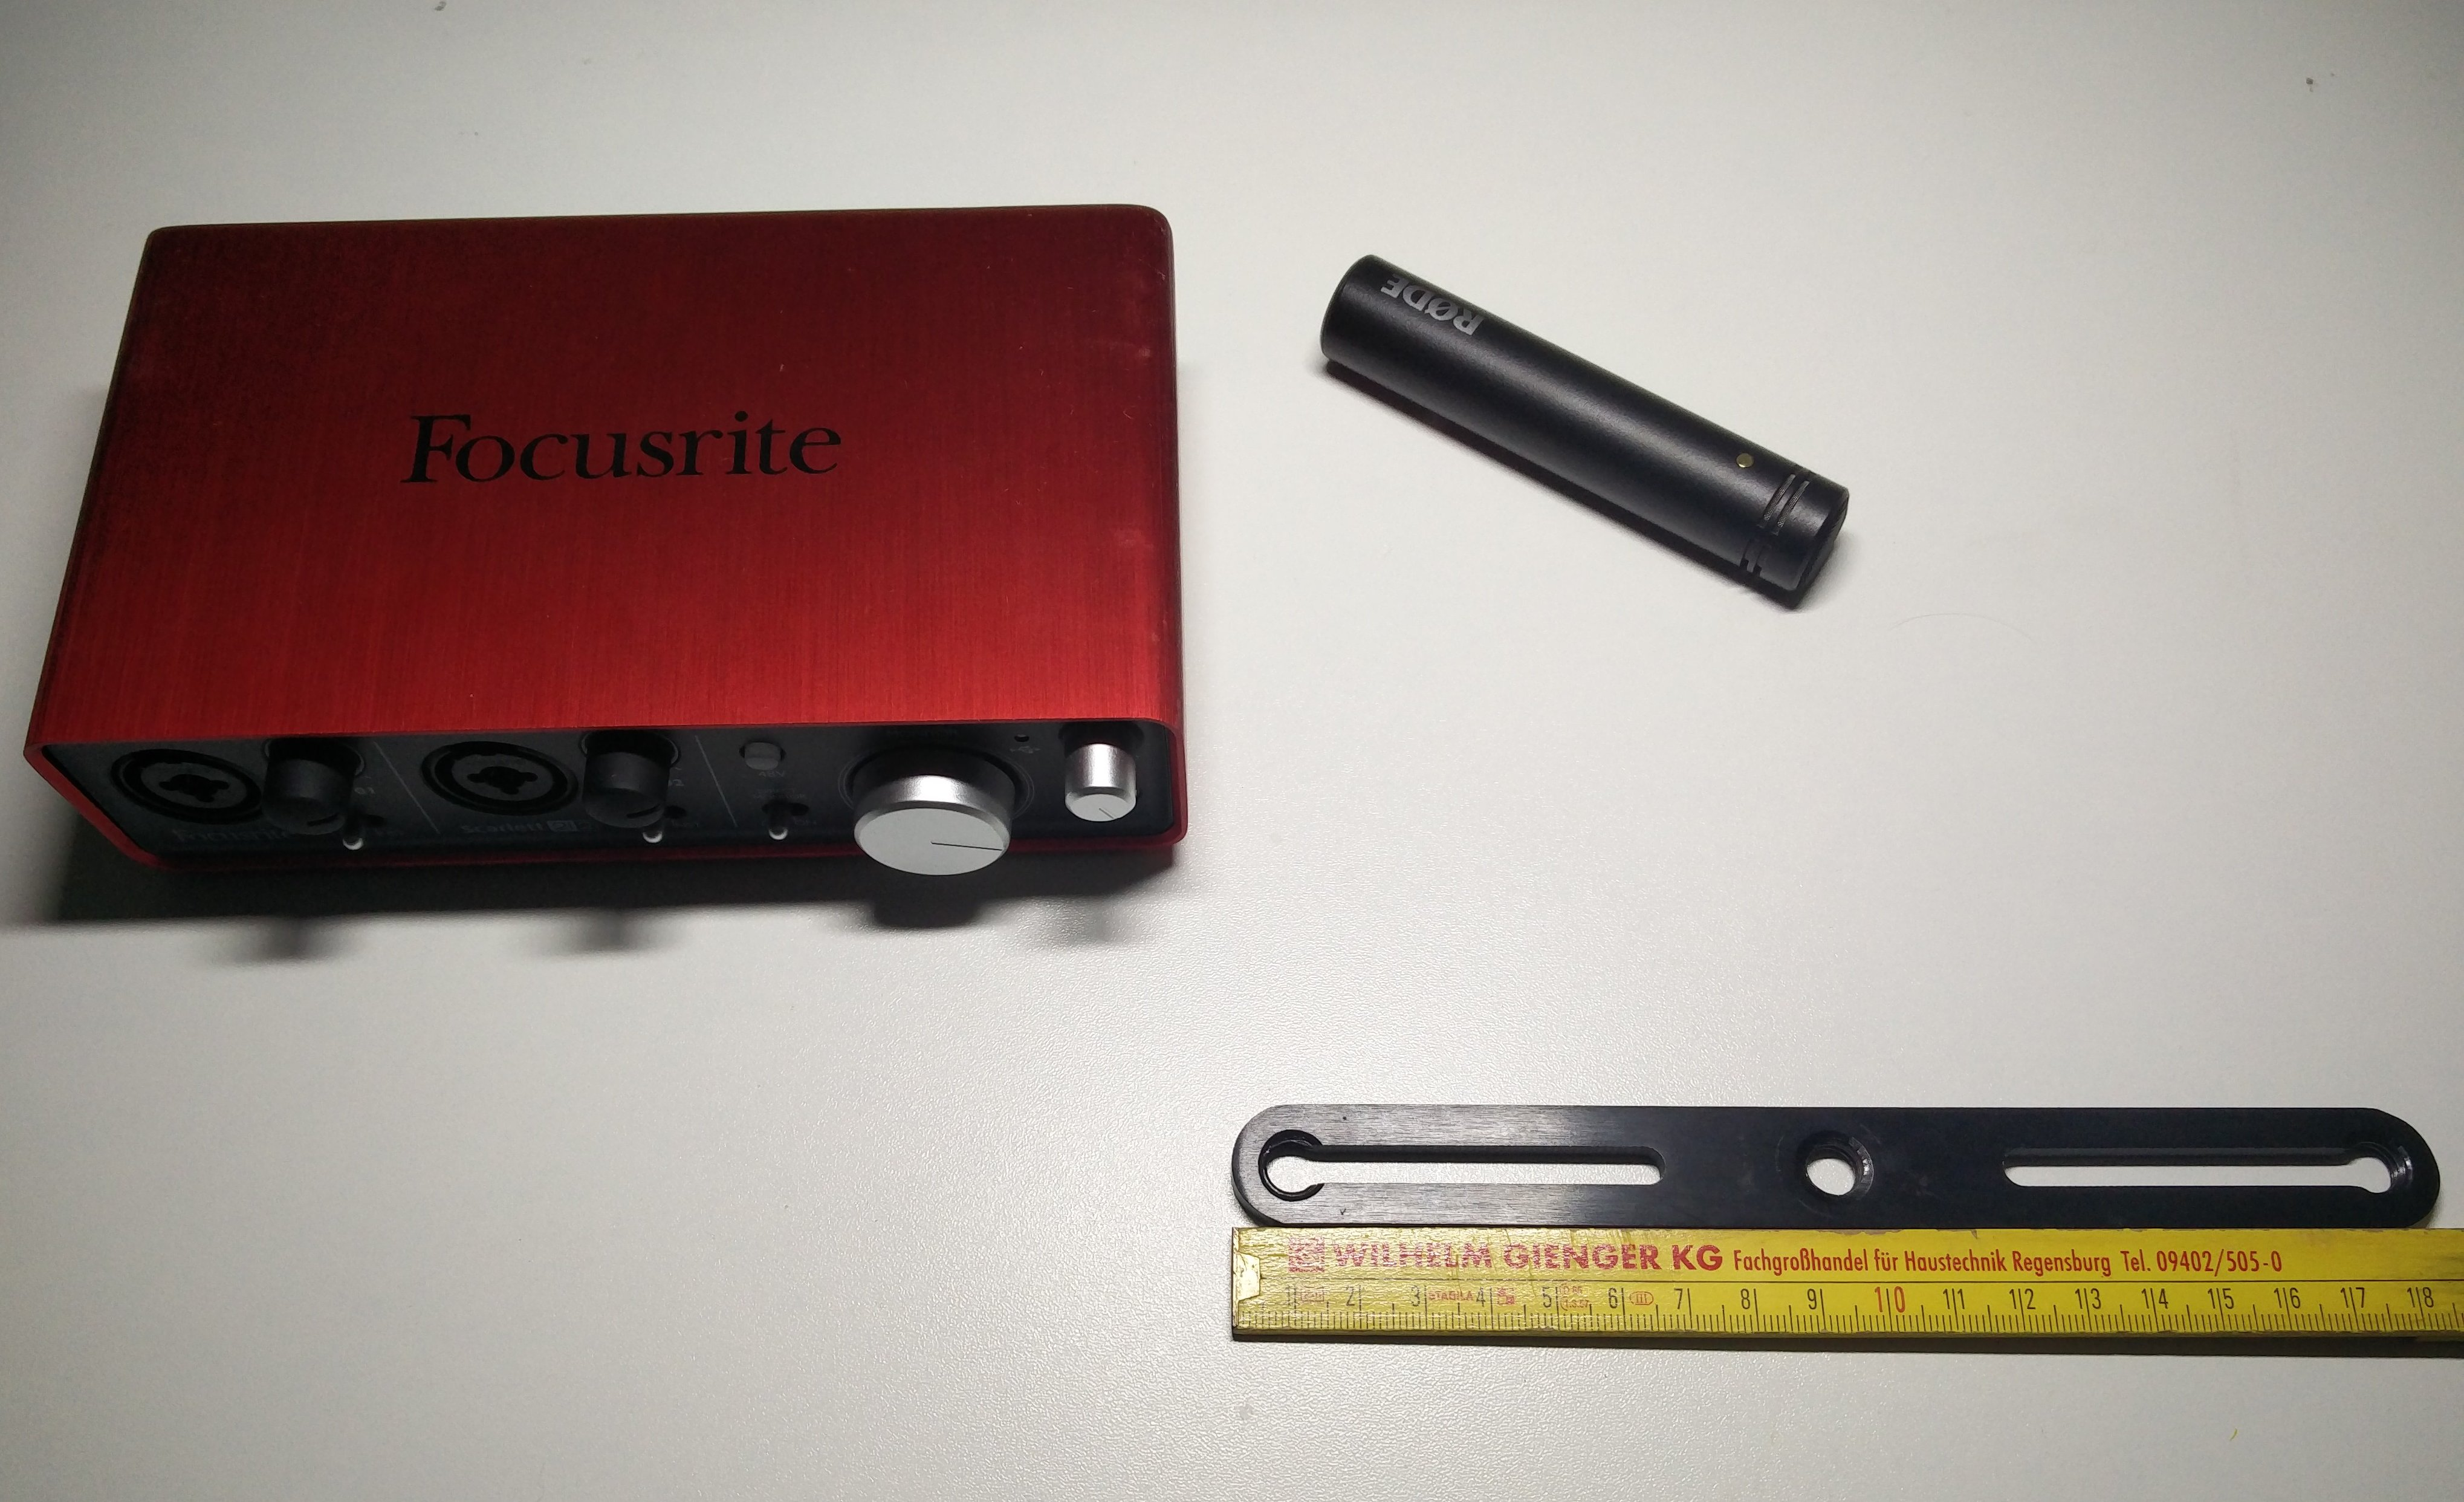
\includegraphics[width=\textwidth]{img/Equipment}
  \caption{Verfügbare Technik}
  \label{material}
\end{figure}

%%%%%%%%%%%%%%%%%%%%%%%%%%%%%%
\section{Programm}
\subsection{Aufbau des Programms}
Das Programm ist in 3 große Teile gegliedert. Dazu zählt das Einlesen der Audiodateien, die benötigte Signalverarbeitung inklusiver Berechnung der gewünschten Parameter und das Speichern der gewonnenen Werte in Form einer Excel-Datei.
\paragraph{Einlesen der Audiodaten}
Die Audiodateien liegen im WAV-Format als Stereoaufnahme vor. Zunächst wird eine Liste mit allen Dateien in einem bestimmten Ordner erstellt, damit die Dateien nacheinander eingelesen werden können. Im nächsten Schritt werden die beiden Kanäle voneinander getrennt, um diese dann in die Signalverarbeitung zu übergeben.
\paragraph{Signalverarbeitung}
Das Kernstück der Signalverarbeitung ist eine periodische Korrelationsfunktion, die den linken und rechten Kanal miteinander korreliert. Die dabei entstandene Korrelationsfunktion wird dann weiter untersucht. Als nächstes wird eine Art Einhüllende berechnet, die ein Maß für die Steilheit der Kurve ist. Wie bereits im Abschnitt 3.3 "Gauß-Regression" beschrieben, wird dann mit Hilfe der Methode der kleinsten Quadrate eine Gauß-Glocke so angepasst, dass sie den Verlauf der Hüllkurve der KKF möglichst gut abbildet. Die Parameter ripple, $\sigma$, Gleichanteil und Zeitverschiebung des Maximums aus dem Ursprung werden danach an eine Funktion übergeben, die diese Daten in einer Excel-Tabelle speichert.
\paragraph{Speicherung}
Die Speicherung der Daten erfolgt in einer Excel-Datei. Dabei wird zu erst der Dateiname des Samples und alles dazugehörigen Werte gespeichert. Außerdem wird noch ein Link zum Graphen der Korrelationsfunktion angegeben, damit man sich diese bei der Auswahl der Test-Signale anschauen kann.

\subsubsection{Programmablaufplan}
\begin{figure}[ht!]
\centering
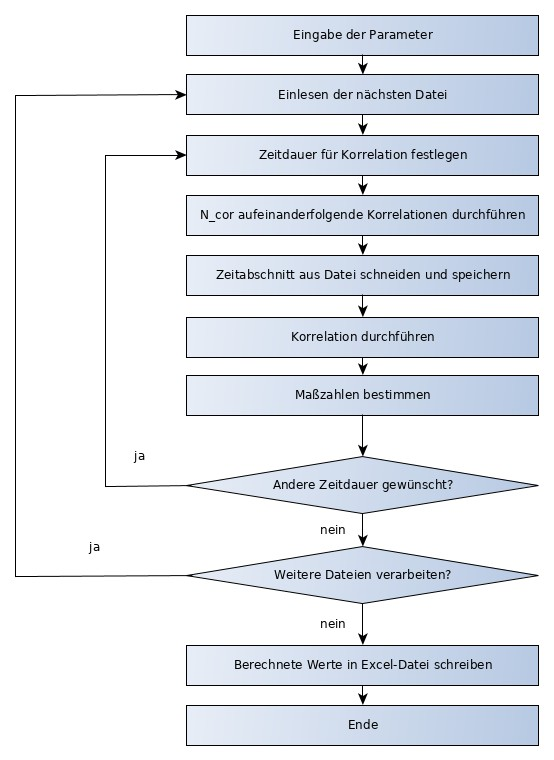
\includegraphics[scale=0.6]{img/pap}
\caption{Programmablaufplan}
\label{figure1}
\end{figure}

\subsection{Mögliche Einstellungen}
Im Code gibt es diverse Eintellungen, die das Verhalten des Programms je nach Wunsch des Anwenders verändern. Diese sind am Beginn der main.m-Datei festgelegt und werden im folgenden beschrieben:
\begin{itemize} 
\item $path$ - Pfad zur Sammlung der WAV-Dateien
\item $excel\_path$ - Pfad unter dem Excel-Datei mit Lösungen gespeichert wird
\item $output$ - Unterscheidung, ob Ergebnisse gespeichert oder angezeigt werden
\item $calc$ - Wechsel zwischen Berechnung im Zeit- und Frequenzbereich möglich.
\item $x\_axes$ - Unterscheidung, ob Korrelation gegen Samples oder Zeit aufgetragen wird
\item $priority$ - Unterscheidung, ob angegebene Blocklänge oder Zeitdauer priorisiert wird
\item $t\_start$ - Startzeitpunkt der Korrelation
\item $t\_dur$ - Array $A1$ mit Menge an Zeitdauern die korrelierten werden sollen, Korrelation beginnt immer bei $t\_start$
\item $Ncor\_init$ - Array, mit identischer Länge zu $A1$. Gibt an wie oft korrespondierender Eintrag in $A1$ hintereinander korreliert wird. 
\item $Lcor$ - Blocklänge der Korrelation
\end{itemize}
\subsection{Probleme} 


%%%%%%%%%%%%%%%%%%%%%%%%%%%%%%
\section{Signalauswahl}
Wir haben für die Aufnahme der Signale viel verschiedene Situationen ausgesucht, um ein möglichst breites Spektrum an Raum-Effekten zu erhalten. Aufnahmeorte waren beispielsweise der Platz vor dem HSZ, die Wiese zwischen Physik- und Mathematikgebäude, sowie der Trefftzbau. Außerdem wurde in einer Wohnung gemessen, um Effekte von schallabsorbierenden Stoffen wie Teppich oder Bett zu erhalten. Soweit mgölich, haben wir die natürliche Geräuschkulisse am jeweiligen Ort eingefangen. Zusätzlich dazu wurde ein definiertes Signal mittels eines Lautsprechers erzeugt, um Direktschall zu nutzen. Bei diesen Aufnahmen sollten die Effekte des Raumes am deutlichsten hervortreten.
\subsection{Beispielsignale}
\subsubsection{Signal 1 - trefftz$\_$wiese$\_$m}
\paragraph{Aufnahmesituation} Dieses Signal wurde auf der Wiese zwischen dem Gebäude der Mathematik- und Physikfakultät aufgenommen. Das heißt, es ist eine relativ große Freifläche mit wenigen Hindernissen mit ungehinderter Schallausbreitung. Es wurde keine zusätzliche Primärschallquelle genutzt.
\paragraph{Signalbeschreibung} Wie in Abbildung \ref{figure2} zu sehen ist, ändern sich beide Kanäle relativ langsam. Sowohl Kanal A als auch Kanal B sind klar definiert und im Vergleich zum Rauschen relativ groß. Man erkennt jedoch bereits beim einfachen Betrachten, dass sich beide Seiten nur sehr geringfügig ähnlich sehen.
\begin{figure}[ht!]
\centering
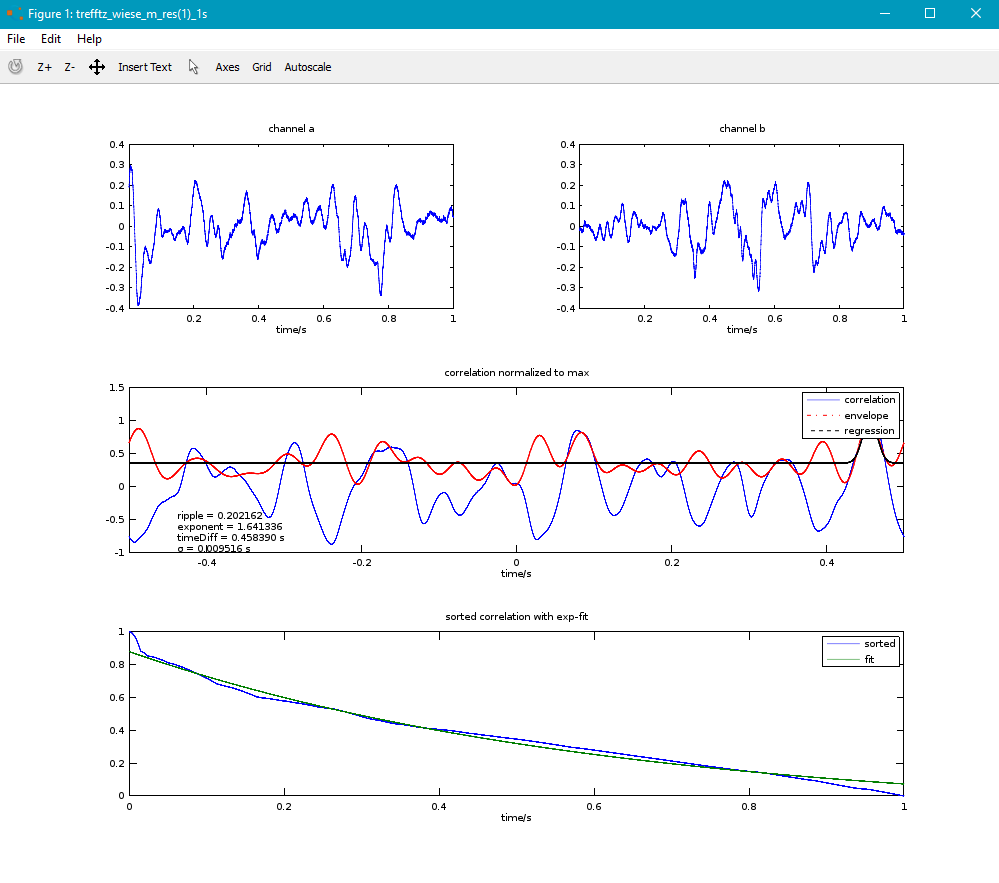
\includegraphics[scale=0.64]{img/trefftz_wiese_m}
\caption{Signal 1}
\label{figure2}
\end{figure}
\paragraph{Beschreibung der KKF} Die Kreuzkorrelationsfunktion schwankt sehr stark über den gesamtem Zeitbereich. Deswegen ist auch die Hüllkurve stark schwankend. Da die Regression über die Hüllkurve berechnet wird, wird diese dem Signal auch nicht gerecht.
\paragraph{Auswertung der Maßzahlen}

\subsubsection{Signal 2 - trefftz$\_$fahrstuhl$\_$m}
\paragraph{Aufnahemsituation} Diese Aufnahme fand im Fahrstuhl des Trefftzbaus statt. Das heißt, der Raum war relativ klein und ist mit schallharten Begrenzungen versehen. Um ein Signal zu erhalten wurde eine Primärschallquelle in Form eines hochwertigen Lautsprechers genutzt.
\paragraph{Signalbeschreibung}
In Abbildung \ref{figure3}  erkennt man sehr gut, dass sich beide Kanäle sehr schnell ändern und einen ähnlichen Verlauf haben. Lediglich die Stärke des Signals ist unterschiedliche. Das stört jedoch nicht für die Berechnung der Maßzahlen. 
\begin{figure}[ht!]
\centering
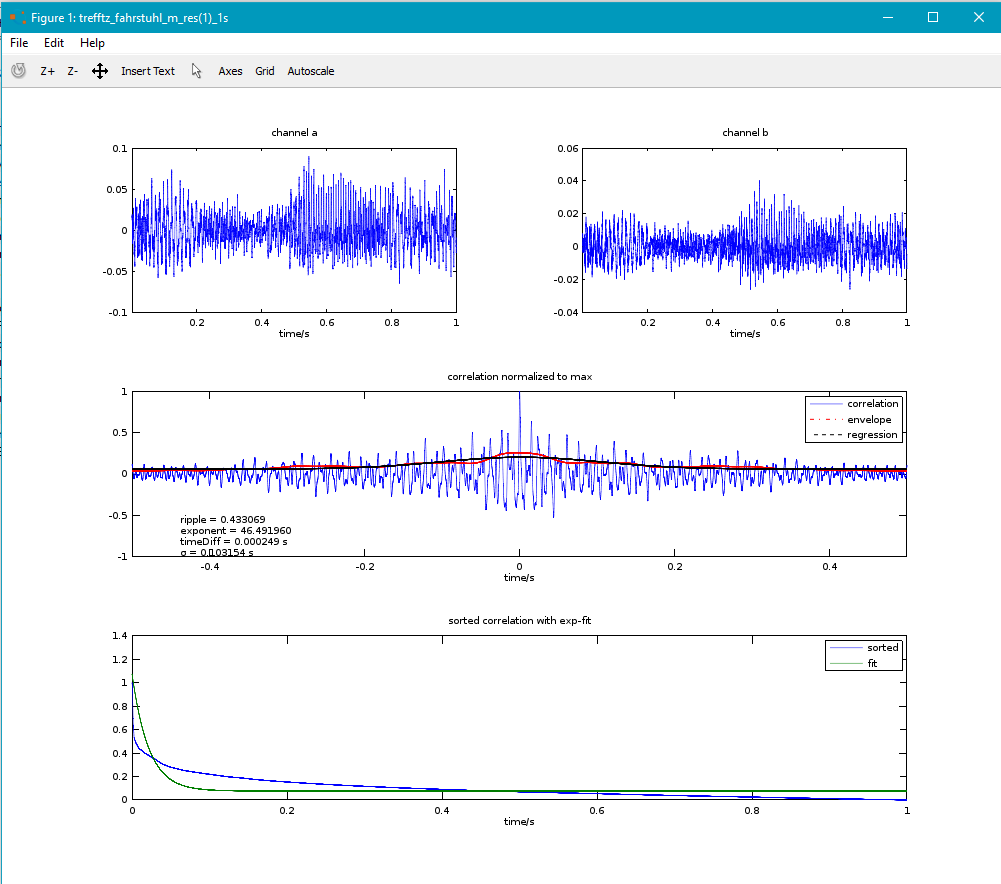
\includegraphics[scale=0.64]{img/trefftz_fahrstuhl_m}
\caption{Signal 2}
\label{figure3}
\end{figure}
\paragraph{Beschreibung der KKF}
Für dieses Signal ist auch an der Kreuzkorrelationsfunktion klar zu sehen, dass es ein Maximum in der Mitte gibt. Das heißt, die Signale sind sich sehr ähnlich. Zu den Seiten nimmt die KKF langsam ab. Für solch einen Verlauf ist die Aussage der Hüllkurve und der Regression sehr gut, da dieses Kreuzkorrelation gut mit einer Gauß-Kurve approxmiert werden kann.
\paragraph{Auswertung der Maßzahlen}

\subsection{Probleme bei der Signalauswahl}
Bei der Signalauswahl ergab sich das Problem, dass man möglichst viele verschiedene Raumsituationen erfassen musste, um möglichst viele verschiedene Daten zu bekommen. Dabei war es jedoch nur schwer möglich vor Ort zu entscheiden, ob die entsprechende Aufnahme sinnvolle Ergebnisse liefert.
In den meisten Situationen war der Lautstärkepegel im Raum zu gering um 20s aufzunehmen, ohne das der Großteil der Aufnahme einfach Rauschen war. Aus diesem Grund haben wir ein zusätzliches Signal erzeugt. Dadurch gibt es jedoch in den meisten Aufnahmen eine Primärquelle, die das Spektrum 

\subsection{Fazit}
Abschließend lässt sich feststellen, dass der Gauß-Fit erst aber einem ripple-Faktor von 0.3 sinnvolle Ergebnisse liefert. Bei Werten kleiner 0.3 ist die Hüllkurve einer Gauß-Kurve zu unähnlich. Es ist jedoch festzustellen, dass die Regression der Exponentialfunktion mit kleiner werdendem ripple besser über der nach Größe sortierten Amplituden liegt.
Es ist empfehlenswert, Signale in Räumen aufzunehmen, die ausreichend klein sind, damit die Raumeffekte Auswirkungen auf das Signal haben. Sonst nimmt man größtenteils rauschen auf, welches sehr geringe Aussagen zulässt.


\section{Zusammenfassung}
Es wurde ein Ocatve-Skript entwickelt mit welchem sich die Kreuzkorrelationsfunktion der beiden Stereo-Kanäle einer Audioaufnahme berechnen lässt. Auf Basis der KKF wurden einige einfache Maßzahlen zur Charakterisierung der Aufnahmen entwickelt. Damit lassen sich für bestimmte Anwendungen Signale zu Testzwecken auswählen.
In Zukunft kann die Software auf bestimmte Anwendungsfälle angepasst werden, in dem neue Regressionsmodelle implementiert werden, die der gewünschen Nutzung der Signale besser gerecht werden.
